\documentclass{beamer}
\usepackage[latin1]{inputenc}

\usetheme{Madrid}
\usecolortheme{default}
\usepackage{amsmath}
\usepackage{amssymb,amsfonts,amsthm}
\usepackage{txfonts}
\usepackage{tkz-euclide}
\usepackage{listings}
\usepackage{adjustbox}
\usepackage{array}
\usepackage{tabularx}
\usepackage{gvv}
\usepackage{lmodern}
\usepackage{circuitikz}
\usepackage{tikz}
\usepackage{graphicx}
\usepackage{gensymb}
\usepackage{physics}

\setbeamertemplate{page number in head/foot}[totalframenumber]

\usepackage{tcolorbox}
\tcbuselibrary{minted,breakable,xparse,skins}



\definecolor{bg}{gray}{0.95}
\DeclareTCBListing{mintedbox}{O{}m!O{}}{%
  breakable=true,
  listing engine=minted,
  listing only,
  minted language=#2,
  minted style=default,
  minted options={%
    linenos,
    gobble=0,
    breaklines=true,
    breakafter=,,
    fontsize=\small,
    numbersep=8pt,
    #1},
  boxsep=0pt,
  left skip=0pt,
  right skip=0pt,
  left=25pt,
  right=0pt,
  top=3pt,
  bottom=3pt,
  arc=5pt,
  leftrule=0pt,
  rightrule=0pt,
  bottomrule=2pt,
  toprule=2pt,
  colback=bg,
  colframe=orange!70,
  enhanced,
  overlay={%
    \begin{tcbclipinterior}
    \fill[orange!20!white] (frame.south west) rectangle ([xshift=20pt]frame.north west);
    \end{tcbclipinterior}},
  #3,
}
\lstset{
    language=C,
    basicstyle=\ttfamily\small,
    keywordstyle=\color{blue},
    stringstyle=\color{orange},
    commentstyle=\color{green!60!black},
    numbers=left,
    numberstyle=\tiny\color{gray},
    breaklines=true,
    showstringspaces=false,
}
\title{10.4.1}
\date{12th october, 2025}
\author{Vishwambhar - EE25BTECH11025}

\begin{document}

\frame{\titlepage}
\begin{frame}{Question}
Find the equations of the tangent and the normal, to the curve $16x^2+9y^2=145$ at the point $\brak{x_1,y_1}$, where $x_1=2$ and $y_1>0$.\\
\end{frame}

\begin{frame}{Let}
Let the point of contact of tangent and conic be $\vec{q}$ and also point of intersection of normal and conic be $\vec{q}$.\\
Given
\begin{align}
    \vec{q}=\myvec{2\\k};k>0
\end{align}
\end{frame}

\begin{frame}{Ellipse}
Let the equation of given ellipse in quadratic form be:
\begin{align}
    \vec{x}^\top V\vec{x}+2\vec{u}^\top\vec{x}+f=0\\
\end{align}
where,
\begin{align}
    V=\myvec{\frac{16}{145}&0\\0&\frac{9}{145}}\\
    \vec{u} = \myvec{0//0}
    f=-1
\end{align}
\end{frame}

\begin{frame}{Tangent}
Since $\vec{q}$ lies on the ellipse:
\begin{align}
    \vec{q}^\top V\vec{q}+f=0\\
    \vec{q} = \myvec{2\\3}
\end{align}
The tangent equation can be given by
\begin{align}
    \brak{V\vec{q}+\vec{u}}^\top\vec{x}+\vec{u}^\top\vec{q}+f=0
\end{align}
\end{frame}

\begin{frame}{Normal}
The normal equation can be given by
\begin{align}
    \brak{V\vec{q}+\vec{u}}^\top R\brak{\vec{x}-\vec{q}}=0\\
    R=\myvec{0&-1\\1&0}
\end{align}
After substituting values we get tangent equation in normal form as:
\begin{align}
    \myvec{\frac{32}{145}\\\frac{27}{145}}^\top\vec{x}-1=0
\end{align}
\end{frame}

\begin{frame}{Cocnlusion}
After substituting values we get normal equation in normal form as:
\begin{align}
    \myvec{\frac{-27}{145}\\\frac{32}{145}}^\top\vec{x}-\frac{42}{145}=0
\end{align}
\end{frame}

\begin{frame}[fragile]
    \frametitle{C Code}
    \begin{lstlisting}
#include <stdio.h>
void give_data(double *A, double *u, double *c, double *p, double *m, double *points){
    A[0] = 16.0/145.0; 
    A[1] = 0; 
    A[2] = 0; 
    A[3] = 9.0/145.0;  
    u[0] = 0; 
    u[1] = 0;
    c[0] = -1;   
    p[0] = 2; 
    p[1] = 3;
    m[0] = 32 * 2;
    m[1] = 18 * 3; 
    points[0] = A[0];
    points[1] = A[3];
    points[2] = c[0];
    points[3] = p[0];
    points[4] = p[1];
}
    \end{lstlisting}
\end{frame}

\begin{frame}[fragile]
    \frametitle{Python code 1}
    \begin{lstlisting}
import ctypes as ct
import numpy as np
from numpy.lib import scimath as np_scimath
lib = ct.CDLL("./problem.so")
lib.give_data.argtypes = [
    ct.POINTER(ct.c_double), ct.POINTER(ct.c_double),
    ct.POINTER(ct.c_double), ct.POINTER(ct.c_double),
    ct.POINTER(ct.c_double), ct.POINTER(ct.c_double)
]
pointsA = ct.c_double * 4
pointsu = ct.c_double * 2
pointsc = ct.c_double * 1
pointsp = ct.c_double * 2
pointsm = ct.c_double * 2
points = ct.c_double * 5
    \end{lstlisting}
\end{frame}

\begin{frame}[fragile]
    \frametitle{Python code 1}
    \begin{lstlisting}
A = pointsA()
u = pointsu()
c = pointsc()
p = pointsp()
m = pointsm()
data = points()
lib.give_data(A, u, c, p, m, data)
A = np.array([[A[0], A[1]], [A[2], A[3]]])
u = np.array([[u[0]], [u[1]]])
p = np.array([[p[0]], [p[1]]])
m = np.array([[m[0]], [m[1]]])
c = c[0]
    \end{lstlisting}
\end{frame}

\begin{frame}[fragile]
    \frametitle{Python code 1}
    \begin{lstlisting}
a1 = float(m.T @ A @ m)
b1 = float(2 * (p.T @ A @ m + u.T @ m))
c1 = float(p.T @ A @ p + 2 * u.T @ p + c)
D = b1**2 - 4 * a1 * c1
t1 = (-b1 + np_scimath.sqrt(D)) / (2 * a1)
t2 = (-b1 - np_scimath.sqrt(D)) / (2 * a1)
A_point = p + t1 * m
B_point = p + t2 * m
def send_data():
    return (data, float(A_point[0]), float(A_point[1]), float(B_point[0]), float(B_point[1]))
    \end{lstlisting}
\end{frame}

\begin{frame}[fragile]
    \frametitle{Python code 2}
    \begin{lstlisting}
import matplotlib.pyplot as plt
from call import send_data
import numpy as np
data, Ax, Ay, Bx, By = send_data()
x = np.linspace(-3.010, 3.010, 2500)
y = np.sqrt(145/9-(16*x**2)/9)
Xt = np.linspace(-5, 5, 100)
Yt = (145/27) * (1 - (32/145)*Xt)
Xn = np.linspace(-5, 5, 100)
Yn = (54/64) * (Xn - 2) + 3
    \end{lstlisting}
\end{frame}

\begin{frame}[fragile]
    \frametitle{Python code 2}
    \begin{lstlisting}
plt.plot(x, y, "r")
plt.plot(x, -y, "r")
plt.plot(Xt, Yt, "g")
plt.plot(Xn, Yn, "b--")

plt.plot(2, 3, "ko")
plt.text(2.1, 3.1, "(2,3)", color="black")
plt.text(2.36, -2.77, r'$16x^2+9y^2=145$', color = "black")
plt.text(-3.04, 9.18, r'$32x+27y=145$', color="black")
plt.text(4.35,4.95,r'$-27x+32y=42$', color="black")
    \end{lstlisting}
\end{frame}

\begin{frame}[fragile]
    \frametitle{Python code 2}
    \begin{lstlisting}
plt.xlabel("X-axis")
plt.ylabel("Y-axis")
plt.axis("equal")
plt.grid(True)
plt.savefig("../figs/plot.png")
plt.show()
    \end{lstlisting}
\end{frame}

\begin{frame}{Plot}
    \begin{figure}
        \centering
        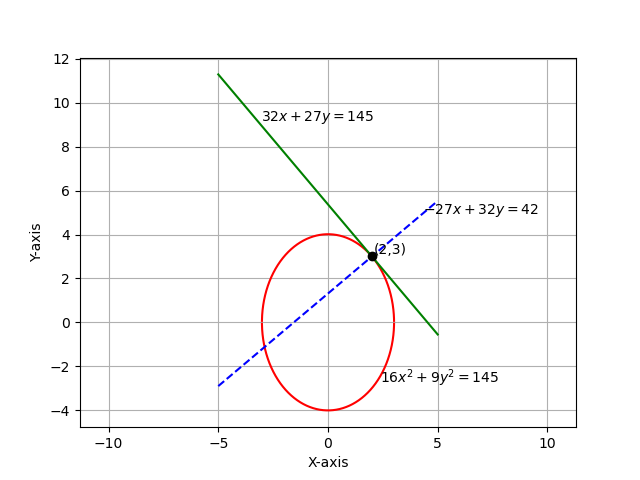
\includegraphics[width=0.5\columnwidth]{../figs/plot.png}
        \caption{Plot of the ellipse, tangent and normal}
        \label{fig:fig}
    \end{figure}
\end{frame}

\end{document}